\section{Pileup jet rates}
\label{sec:pileupjetrates}
Figure~\ref{fig:PUJetRate_pt20} shows the mean number of pileup jets with $\pT > 20\GeV$ per event  
for two different bin in pseudorapidity: $|\eta|<2.4$ and $2.4<|\eta|<4.5$. 
No cuts are imposed to suppress pileup jets. An approximately quadratic increase of the pileup jet multiplicity with the average
number of interactions per bunch crossing $\mu$ is observed. 
\label{sec:Appendix_PUjetRates}
\begin{figure}[!htbp]
  \centering
  \subfigure[]{
      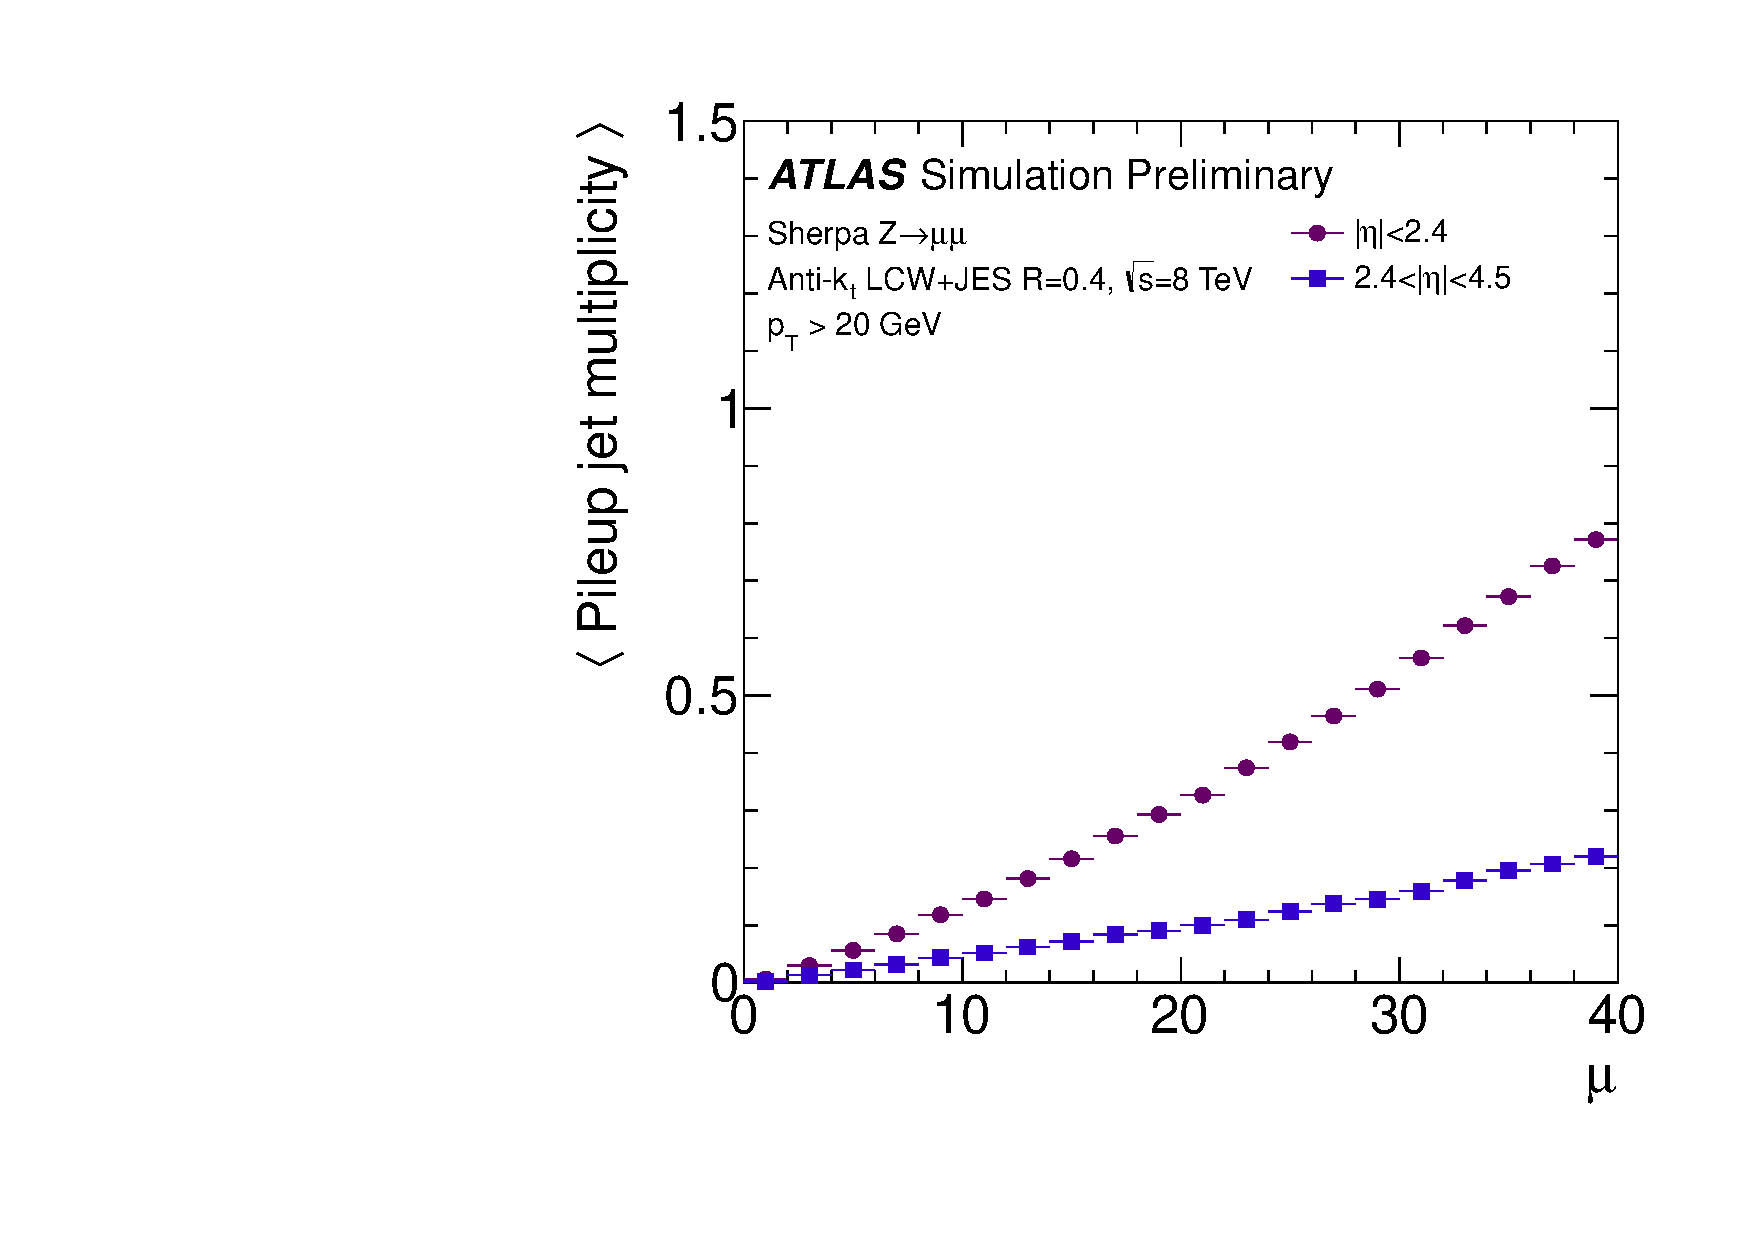
\includegraphics[width= 0.46\textwidth]{PileupJetRateVsEta_Pt20}
    \label{fig:PUJetRate_pt20}
  }
  \subfigure[]{
      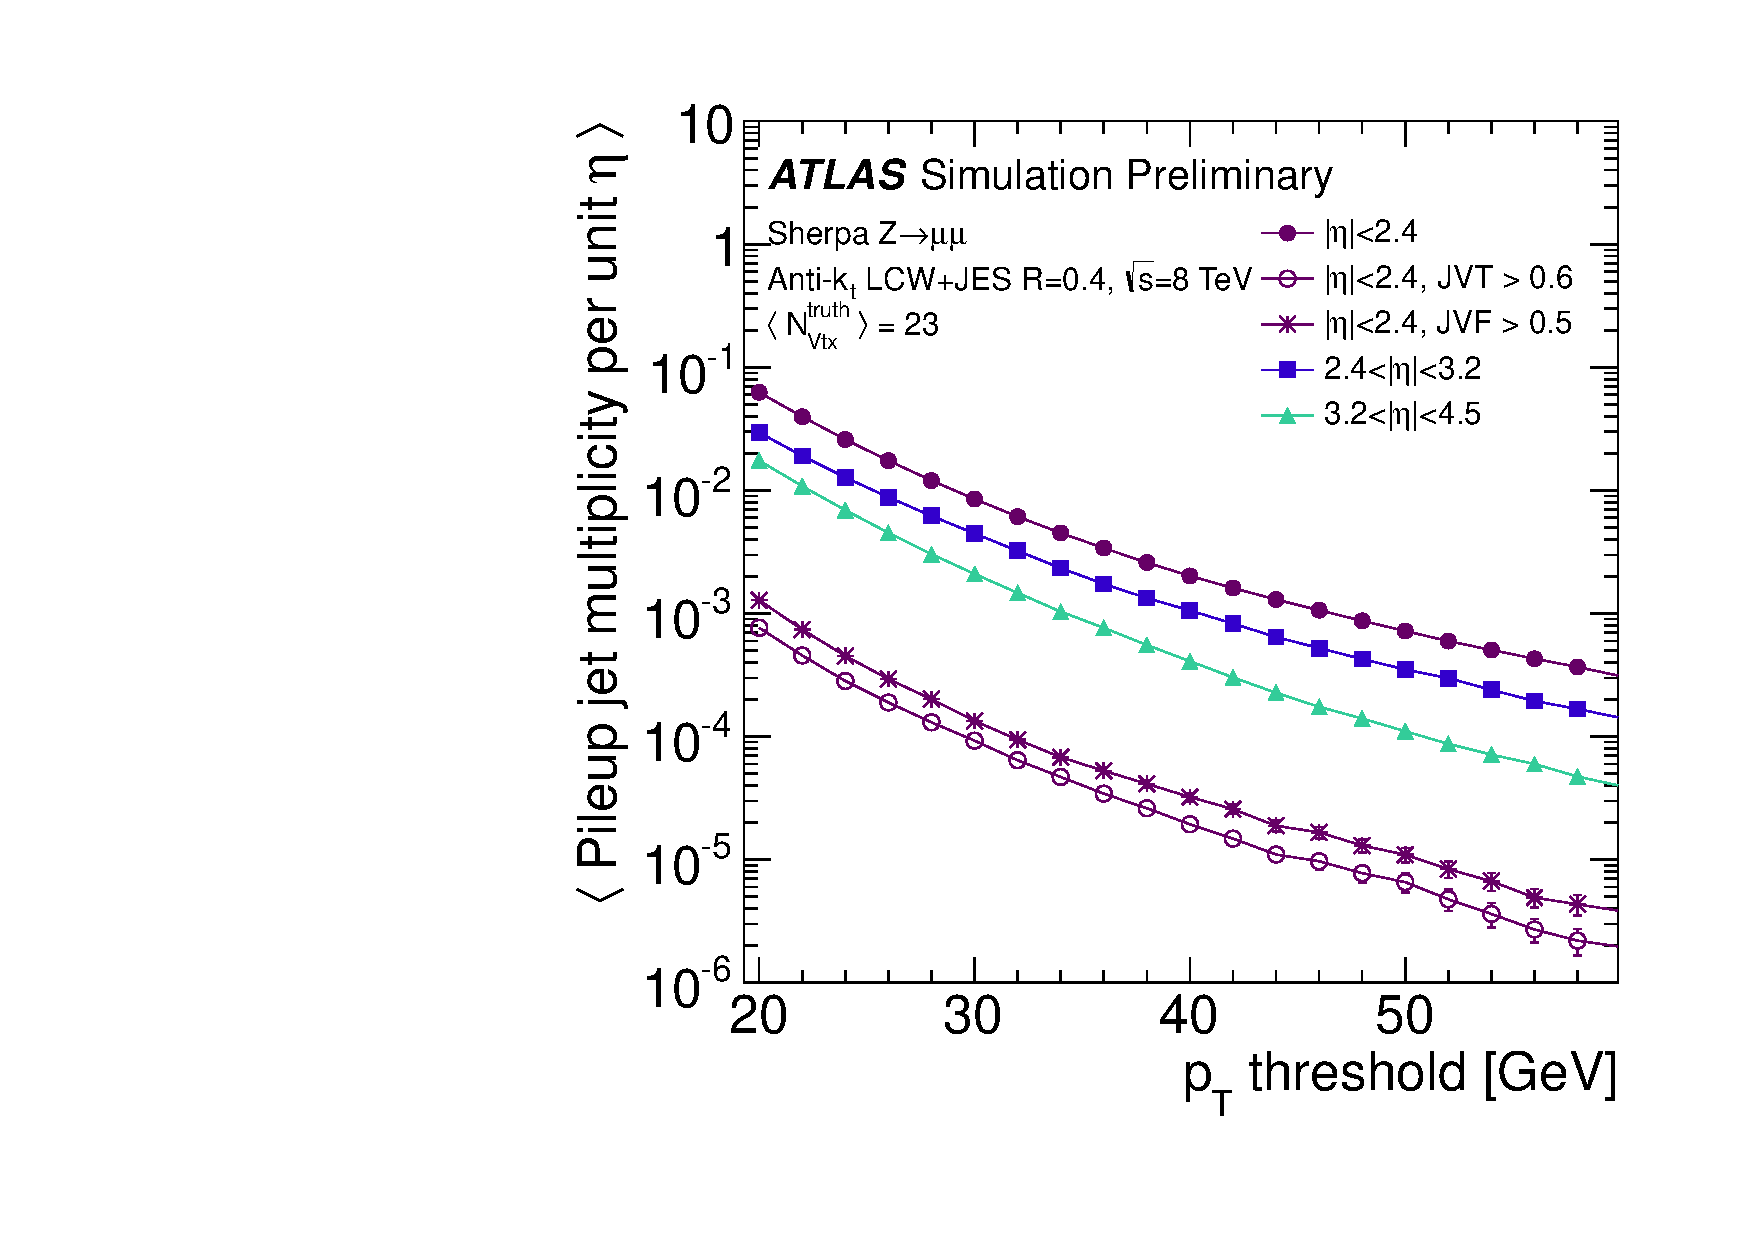
\includegraphics[width=0.46\textwidth]{PileupJetRateVsEtaVsPt}
    \label{fig:PUJetRate_vsPtvsEta}
  }
  \caption{(a) Mean number of pileup jets with $\pT>20\GeV$ as a function of $\mu$. (b) Pileup jet multiplicity per unit $\eta$ as a function of 
  \pT threshold for different regions of pseudorapidity.
  }
\label{fig:PUJetRates}
\end{figure}
Figure~\ref{fig:PUJetRate_vsPtvsEta} shows the pileup jet multiplicity per unit $\eta$ as a function of jet \pT threshold for different $\eta$ regions. 
The pileup jet rates in the forward regions of the detector are largely suppressed with respect to the $|\eta|<2.4$ central region. 
The graphs with magenta stars and open circles represent respectively the pileup jet rates after imposing $\JVF > 0.5$ and $\JVT > 0.6$ criteria
to suppress pileup jets in the cental region. The chosen cut values for \JVF and \JVT both result in hard-scatter jet efficiencies of 
about 85\% and 90\% for jets with $20<\pT<30\GeV$ and $30<\pT < 40\GeV$. 
